\newcommand{\mkbibnodate}{n\adddot d\adddot}
\section{Einleitung}
%for reference to this section
\label{section:Einleitung}

\subsection{Forschungsgebiet}
\subsection{Relevanz}
\subsection{Forschungsfrage}
\subsection{Aufbau der Arbeit}

\section{Die Taratoga Formel}

Text mit beliebigen Sonderzeichen in UTF-8 ohne BOM, 
\textbf{hervorgehobener Text},
\texttt{computerFunction}, kleine mathematische Formel im Text $\sum_{i=0}^n i^2$
\ldots

\subsection{Querverweie, Literaturverweise, Fußnoten}
Für die in Kapitel \ref{section:Einleitung} definierte Forschungsfrage
ist der Begriff \textbf{Taratoga} zentral. In diesem Kapitel wird
der Begriff definiert.

Taratoga\footnote{Taratoga ist ein Wort aus den Sterntagebüchern von Stanislaw Lem} wird in der Informatik
seit den 1970er Jahren in diskutiert in \autocites{McConnell:2004}{Vandevoorde:2002},
das Standardwerk, das auch in der Lehre verwendet wird, ist 
\autocite{Tanenbaum:2003}.

Eine erste kompakte Definition findet man bei Renaud: 

\selectlanguage{english}
\begin{quote}
``This quote is completele made up. ... If you do this (make up quotes)
it will end badly for you. ''
\autocite[S.305]{Renaud:2004}
\end{quote}

\textcite{Souders:2007} hat gemessen, dass Performance-Probleme von Webseiten oft im Frontend liegen.
Wenn wir ihn so zitieren, wollen wir seinen Namen nicht in der Klammer haben, sondern davor. das geht
mit \texttt{textcite} statt \texttt{autocite}.

Besonders praktisch sind RFCs zu zitieren: wir haben ein vollständiges
BibTeX-File für alle, und können damit HTTP definieren autocite{rfc1945} <-- Bibtex file korrigieren! TODO ;).

Achtung: nur zitierte Literatur wird im Literaturverzeichnis angeführt.

Wie soll man mit Doku zu einem verwendeten Produkt umgehen?
Entweder in eine Fußnote verbannen, wie die \LaTeX\ Dokumentation\footnote{http://en.wikibooks.org/wiki/LaTeX},
oder richtig zitieren wie \autocite[]{jQueryDoc}.

Manchmal handelt der Text von URLs, zum Beispiel um zu
beschreiben wie http oder https in einer URL wie 
\url{http://example.com} verwendet werden.

Die Wikipedia ist immer der \textbf{Anfang}  einer Recherche, 
nicht das Ende. Für Neben-Themen ist sie aber ganz praktisch, 
man kann zum Beispiel für BibTeX und LaTeX darauf verweisen \autocites[BibTeX]{wikipedia:bibtex}[LaTeX]{wikipedia:latex}.

\subsection{Quellen-Arten}

\begin{enumerate}
\item in einem Buch \autocite[580-605]{Tanenbaum:2003}
\item ein Artikel in einem Journal \autocite{Renaud:2004}
\item eine Artikel aus einem Proceedingsband \autocite{Bailey:1981}
\item eine Beitrag auf einer Konferenz ohne richtig veröffentlichen Proceedingsband \autocite{Yacoub:1998}
\item ein RFC autocite{rfc1945} <-- Bibtex file korrigieren!!! TODO ;)
\item eine Bachelorarbeit bei MMT \autocite{Schmidt:2011}
\end{enumerate}


\subsection{Bilder, Diagramme, Grafiken}

% h = try to place the figure Here
% t = try to place the figure at the Top of a page
% p = try to place this figure along with others on a separate Page
% Note that LaTeX has a sophisticated ranking algorithm to place figures.
% It is not always easy to accept LaTeX's placing but it is harder doing it
% manually. Just let it go ;-)
\begin{figure}[h]
	\centering
	\subfloat[Das Julia Fraktal]{
		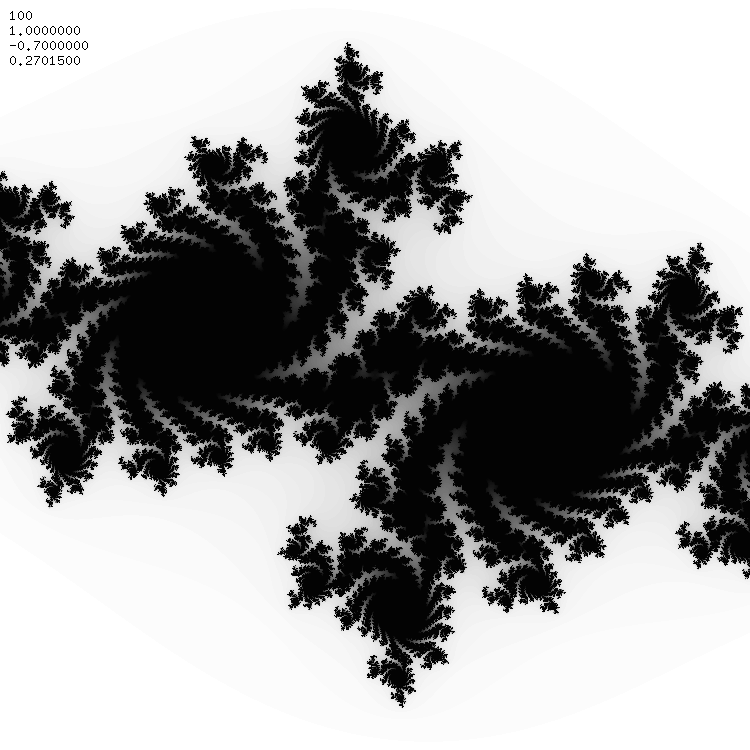
\includegraphics[height=5.0cm]{images/Julia-Fractal.png}
		%for reference of this subfigure only
		\label{subfigure:Julia-Fractal}
	}
	\qquad
	\subfloat[Noise für Tinteneffekte]{
		
\includegraphics[height=5.0cm]{images/Perlin-Coherent.png}
		%for reference of this subfigure only
		\label{subfigure:Perlin-Coherent}
	}
	\caption[
		Verschiedene Pixelgraphiken\newline
		% source url given in the table of figures
		\small\texttt{https://mediacube.at/wiki/}
	]{
		Verschiedene Pixelgraphiken
	}
	%for reference to all subfigures
	\label{figure:PixelImages}
\end{figure}

Unterstützte Pixelgraphikformate: PNG, JPEG, PDF.
Angabe von height oder width meist wichtig.

Jede Abbildung die Sie zeigen erkläutern Sie auch im Text. Dabei verweisen Sie auf die
Abbildung mit \texttt{\\ref}. Abbildung \ref{figure:PixelImages} stellt zwei Bilder gegenüber,
ohne dass das Sinn macht.  Unterabbildung \ref{subfigure:Julia-Fractal} zeigt einen
Ausschnitt aus dem Julia-Fraktal in der schwarz-weiss Darstellung.

\begin{figure}[h]
	\centering
	
\includegraphics{images/KappaGamma.pdf}
	\caption{
		Vektorgraphik mit \LaTeX\ Beschriftung ($\kappa$, $\gamma$)
	}
	%for reference to this figure
	\label{figure:KappaGammaTau}
\end{figure}

Referenz auf Abbildung \ref{figure:KappaGammaTau}.

Bei Vektorgraphik mit \LaTeX\ Beschriftung keine Skalierung mit width
oder height verwenden!
Vektorgraphik mit \LaTeX\ Beschriftung kann etwa mit \texttt{ipe} erstellt
werden.

Unterstütztes Vektorgraphikformat: PDF. EPS muss konvertiert werden.


\subsection{Codebeispiele, etc}
%for references to this subsection
\label{subsection:Coding}

\begin{lstlisting}[
	label=listing:Main, %for reference to this listing
	float=h,
	caption=main.cpp,
	firstnumber=10
]
int main(void) {
	while (true) {
	}
	return 0;
}
\end{lstlisting}

Referenz zu Listing \ref{listing:Main}.

Bei Codeausschnitten immer die erste Zeilennummer passend zum File angeben.

\begin{lstlisting}[
	float=h,
	caption=Select Abfrage in SQL,
	language=SQL
]
	SELECT * FROM users WHERE id = 1;
\end{lstlisting}


\subsection{Aufzählerei}

\begin{enumerate}
	\item Punkt 1
	\begin{enumerate}
		\item Unterpunkt 1
		\item Unterpunkt 2
	\end{enumerate}
	\item Punkt 2
\end{enumerate}

\begin{itemize}
	\item Punkt 1
	\begin{itemize}
		\item Unterpunkt 1
		\item Unterpunkt 2
	\end{itemize}
	\item Punkt 2
\end{itemize}


\subsection{Tabelle}

\begin{table}[h]
	\centering
	\begin{tabular}{r|rrr}
		    & $i$ & $j$ & $k$ \\ \hline
		$i$ &$-1$ & $k$ &$-j$ \\
		$j$ &$-k$ &$-1$ & $i$ \\
		$k$ & $j$ &$-i$ &$-1$
	\end{tabular}
	\caption{
		Multiplikationstabelle für Quaternionen
	}
	\label{table:Quaternions}
\end{table}

Referenz auf Tabelle \ref{table:Quaternions}.

\section{Formeln}
\label{section:MathematicalStuff}

Sei $f(x)$ eine stetige Funktion, so ist die \textbf{Fourier Transformierte}
$F(\omega)$ wie folgt definiert:
\begin{equation}
\label{equation:FourierDefinition}
	F(\omega) = \int_{-\infty}^{\infty} f(x) e^{-i\omega t} dt
\end{equation}

Referenz auf mathematische Gleichung (\ref{equation:FourierDefinition}).

Unnummerierte Gleichung:
\begin{equation*}
	e^{i\varphi} = \cos\varphi + i \sin\varphi
\end{equation*}
%you may also use \[ \] instead of \begin{equation*} and \end{equation*}

Gleichungssystem:
\begin{eqnarray}
	g(x) = f(x - x_0) & \Leftrightarrow &
		G(\omega) = F(\omega) e^{-i\omega x_0} \\
	g(x) = f(x) e^{i\omega_0 x} & \Leftrightarrow &
		G(\omega) = F(\omega - \omega_0)
\end{eqnarray}
